\section{Experiment}
\label{sec:experiment}
\subsection{Experimental Setup}
\subsubsection{Dataset Configurations}
The experiments are performed on the collected dataset, which comprises 5,000 examples in total. We use 4,500 examples for training and 500 for testing. The same 500 test examples are used in all three assessment forms (SCQ, MCQ, and TFQ), instantiated via prompt templates for textual, numerical or visual inputs.

\subsubsection{Comparison Models}
We evaluate three categories of models under the GWC framework, aligned with Table~\ref{tab:main_results_hierarchical}.

\textbf{General (zero-shot).} No task-specific training on dataset. \textit{Textual and numerical modality:} Llama-3.3-70B-Instruct, Llama-3.2-1B, Qwen2.5-3B, Mistral-Small-24B-Instruct. \textit{Visual modality:} LLaVA-1.5-7B, Qwen2-VL-2B, Gemma-3-27B-IT \cite{team2023gemini}, Ministral-14B-Instruct.

\textbf{Lightweight (ours).} Trained from scratch on MatchIntel2. \textit{Numerical modality:} 1D CNN. \textit{Visual modality:} MIL-ResNet-18.

The full training protocol (input formatting, PEFT, lightweight architectures, and hyperparameters) is given in Appendix~\ref{sec:training-protocol}.



\begin{table*}[t]
    \centering
    \caption{Comprehensive performance comparison on numerical and visual modalities. Models within each modality are categorized into General (Zero-Shot), Fine-Tuned, and Lightweight architectures. Accuracy is evaluated on MCQ, SCQ, and TFQ. $\dagger$ denotes theoretically calculated values.}
    \label{tab:main_results_hierarchical}
    \renewcommand{\arraystretch}{1.2} % 保持舒展的行高
    \setlength{\tabcolsep}{14pt} % ⭐ 核心魔法：将默认的列间距统一放大，让表格大气但不割裂
    \begin{tabular}{@{} l l c c c c @{}}
        \toprule
        \multirow{2}{*}{\textbf{Category}} & \multirow{2}{*}{\textbf{Model}} & \multirow{2}{*}{\textbf{Params}} & \multicolumn{3}{c}{\textbf{Accuracy (\%)}} \\
        \cmidrule(lr){4-6} 
        & & & \textbf{MCQ} & \textbf{SCQ} & \textbf{TFQ} \\
        \midrule
        
        % ==========================================
        % 基线部分
        % ==========================================
        Baseline & Random-Level & - & 12.95$^\dagger$ & 30.81$^\dagger$ & 56.74$^\dagger$ \\
        \midrule
        
        % ==========================================
        % 文本模态
        % ==========================================
        \multicolumn{6}{c}{\textit{Textual Modality}} \\
        \midrule

        \multirow{4}{*}{General (Zero-Shot)} 
         &  GPT-5.4 & - & $15.00 \pm 3.16$ & $36.20 \pm 4.87$ & $54.23 \pm 5.11$ \\
        & Claude-4.6-opus & - & $14.40 \pm 2.06$ & $33.20 \pm 4.53$ & $53.54 \pm 2.28$ \\
        & Llama-3.1  & 70B & $11.60 \pm 3.26$ & $35.60 \pm 6.62$ & $53.47 \pm 6.30$  \\
        & Mistral-Small-3 & 24B & $9.00 \pm 4.20$ & $33.60 \pm 5.95$ & $50.89 \pm 3.81$ \\
        & Qwen-2.5  & 3B & $7.20 \pm 2.71$ & $20.80 \pm 5.11$ & $38.13 \pm 6.72$ \\
        & vicuna-1.5  & 7B & $8.40 \pm 1.36$ & $14.60 \pm 1.62$ & $50.00 \pm 0.00$ \\
        \cmidrule(l){2-6} 
        
        \multirow{2}{*}{Lightweight (Ours)} 
        & \textbf{LSTM} & 4.60M &  $20.00 \pm 3.85$ & $ 37.20 \pm 4.07$ & $61.74 \pm 2.27$ \\
        & \textbf{MLP} & 3.98M & $17.20 \pm 1.47$ & $ 33.60 \pm 2.24$ & $58.28 \pm 2.77$ \\
        & \textbf{GRU} & 4.44M & $21.00 \pm 2.28$ & $ 36.60 \pm 3.79$ & $60.05 \pm 2.26$ \\
        \midrule

        % ==========================================
        % 数字模态
        % ==========================================
        \multicolumn{6}{c}{\textit{Numerical Modality}} \\
        \midrule
        
        \multirow{4}{*}{General (Zero-Shot)} 
        &  GPT-5.4 & - & $10.40 \pm 2.94$ & $33.40 \pm 6.89$ & $54.22 \pm 6.22$ \\
        & Claude-4.6-opus & - & $14.40 \pm 3.61$ & $36.40 \pm 8.27$ & $56.36 \pm 8.92$  \\
        & Llama-3.1  & 70B & $6.40 \pm 2.42$ & $25.40 \pm 5.54$ & $54.21 \pm 8.67$ \\
        & Mistral-Small-3 & 24B & $5.80 \pm 2.64$ & $22.40 \pm 4.88$ & $53.03 \pm 4.53$ \\
        & Qwen-2.5  & 3B & $6.00 \pm 0.63$ & $24.80 \pm 3.37$ & $36.84 \pm 5.95$ \\
        & vicuna-1.5  & 7b & $12.40 \pm 1.74$ & $13.80 \pm 0.98$ & $50.00 \pm 0.00$ \\
        \cmidrule(l){2-6} 
        
        \multirow{2}{*}{Lightweight (Ours)} 
        & \textbf{CNN} & 0.40M & \textbf{$23.80 \pm 3.31$} & \textbf{$ 36.80 \pm 4.71$} & \textbf{$63.38 \pm 5.65$} \\
        & \textbf{MLP} & 0.43M & \textit{$28.40 \pm 4.22$} & \textit{$38.80 \pm 6.68$} & \textit{$63.87 \pm 4.37$} \\
        & \textbf{GRU} & 0.25M & \textit{$24.00 \pm 4.82$} & \textit{$32.40 \pm 5.78$} & \textit{$60.48 \pm 3.48$} \\
        \midrule
        
        % ==========================================
        % 图像模态
        % ==========================================
        \multicolumn{6}{c}{\textit{Visual Modality}} \\
        \midrule
        
        \multirow{4}{*}{General (Zero-Shot)} 
        &  GPT-5.4 & - & $8.60 \pm 0.49$ & $26.80 \pm 2.56$ & $52.02 \pm 2.39$ \\
        & Claude-4.6-opus & - & $11.40 \pm 1.36$ & $30.60 \pm 5.00$ & $56.59 \pm 3.55$ \\
        &  Llama-3.2-Vision & 90B &  $7.60 \pm 1.36$ & $21.00 \pm 2.28$ & $32.55 \pm 4.28$  \\
        & Mistral-Small-3.1 & 24B & $9.00 \pm 3.63$ & $30.20 \pm 4.26$ & $55.00 \pm 1.89$ \\
        & Qwen-2.5-VL  & 3B & $12.00 \pm 2.19$ & $14.80 \pm 3.76$ & $49.26 \pm 5.52$ \\
        & LLaVa-1.5  & 7B & $5.40 \pm 0.49$ & $13.40 \pm 2.58$ & $50.00 \pm 0.00$  \\
        \cmidrule(l){2-6}
        
        \multirow{2}{*}{Lightweight (Ours)} 
        & \textbf{ResNet-18} & 11.31M & \textbf{$21.40 \pm 2.58$} & \textbf{$35.00 \pm 5.40$} & \textbf{$62.26 \pm 5.33$} \\
        & \textbf{DenseNet-121} & 7.22M & \textbf{$23.20 \pm 2.79$} & \textbf{$35.20 \pm 4.71$} & \textbf{$60.47 \pm 2.26$} \\
        & \textbf{EfficientNet-B0} & 4.34M & \textbf{$24.40 \pm 2.94$} & \textbf{$37.60 \pm 4.72$} & \textbf{$63.11 \pm 1.85$} \\
        
        \bottomrule
    \end{tabular}
\end{table*}


\subsection{Experimental Results and Analytical Insights}
\label{phenomenon}

Table 1 presents a comprehensive performance comparison across textual, numerical, and visual modalities, encompassing general-purpose large models (including state-of-the-art closed-source models and large-scale open-weights models) alongside lightweight task-specific architectures. The empirical data intuitively reveals several highly counter-intuitive phenomena exhibited by current Large Language Models (LLMs) when confronting complex physical world representations.

\textbf{The Inverse Scaling Phenomenon}
Contemporary AI development relies heavily on Scaling Laws, which posit that model capabilities scale monotonically with parameter count. However, our experimental results reveal a highly counter-intuitive "inverse scaling" phenomenon. In the numerical modality, for instance, Llama-3.1 (70B) and Mistral-Small-3 (24B) yield MCQ accuracies of 6.40\% and 5.80\%, respectively. Not only are these performances inferior to the significantly smaller Vicuna-1.5-7B (MCQ: 12.40\%), but they are also comprehensively dominated by a simple CNN architecture with a mere 0.40M parameters (MCQ: 23.80\%) by a margin of over three times. Similarly, in the visual modality, the 90B-parameter Llama-3.2-Vision falls far behind the 4.34M-parameter EfficientNet-B0 in accuracy. This stark contrast—where million-parameter networks absolutely suppress hundred-billion-parameter LLMs—intuitively demonstrates that when confronting specific structural regularities of the physical world, merely scaling up parameters results in computational redundancy rather than the emergence of genuine problem-solving capabilities.

\textbf{Hallucination and Fragility of LMs}
The Mean ± Std (mean and standard deviation) reported in the table reflects not only the absolute performance but also directly exposes the stability and epistemic certainty of the model outputs. Observing the data for general LLMs reveals that they are pervasively accompanied by exceptionally high standard deviations across various physical tasks. For instance, Llama-3.1 70B scores 54.21\% ± 8.67\% on the numerical TFQ task, and Claude-4.6-opus even reaches 56.36\% ± 8.92\%. Such drastic performance fluctuations (with standard deviations reaching 8-9 percentage points) directly expose the extreme Logical Fragility underlying these LLMs. Their representational outputs are highly susceptible to random noise in the input context or minor perturbations in the prompt, essentially degenerating into severe hallucination and random guessing. In contrast, lightweight models (e.g., ResNet-18, EfficientNet-B0) consistently exhibit not only higher means but also significantly lower variances (e.g., EfficientNet-B0 achieving 63.11\% ± 1.85\% on visual TFQ). This proves that architectures equipped with appropriate inductive biases can formulate robust and deterministic reasoning logic when addressing physical tasks.






\subsection{Capability Collapse of LMs Across Multimodalities}
GPT-5.4 and Claude-4.6-opus represent the capability upper bound of current Large Models (LMs). However, this perceived "ceiling" faces a catastrophic failure under our evaluation framework across all task formats. Empirical data reveals that these apex models frequently fail to even reach the mathematical probability of random chance, regardless of whether they are evaluated on the highly challenging MCQ (theoretical random baseline 12.95\%), the intermediate SCQ (30.81\%), or the binary TFQ (56.74\%). Using the visual modality as a diagnostic lens, GPT-5.4 scores a mere 8.60\% on MCQ, 26.80\% on SCQ, and 52.02\% on TFQ—falling strictly below the pure random guessing threshold across all three metrics. Claude-4.6-opus exhibits a similarly dismal and comprehensive collapse (MCQ: 11.40\%, SCQ: 30.60\%, TFQ: 56.59\%).

More crucially, even within their native and most proficient textual modality, the performance of these top-tier models remains fundamentally constrained. While GPT-5.4 and Claude-4.6-opus barely manage to cross the random baseline on textual MCQ and SCQ, they persistently fall below the baseline on TFQ (e.g., GPT-5.4: 54.23\%, Claude-4.6-opus: 53.54\%). Furthermore, they are comprehensively outperformed by the traditional lightweight LSTM architecture across the entire metric matrix (LSTM achieving MCQ: 20.00\%, SCQ: 37.20\%, TFQ: 61.74\%). This persistent cross-modal degradation intuitively proves that the capability collapse of LMs on heterogeneous physical world tasks is not an accidental byproduct of format complexity or insufficient training. On the contrary, it exposes that the entire "autoregressive next-token prediction" paradigm itself inherently possesses an insurmountable capability ceiling.








% To establish the baseline physical-world cognitive capacity and evaluate the \textit{Modality-Agnostic} property, we analyze the zero-shot performance of General LMs against our specialized lightweight architectures across all three modalities. The comprehensive results, detailed in Table \ref{tab:main_results_hierarchical}, yield four critical insights regarding Gestalt World-Level Capability (GWC):

% \textbf{1. The Deficit of High-Level Cognition in Non-Semantic Environments.}
% The most striking observation is the catastrophic failure of state-of-the-art general models when confronted with raw, non-semantic physical observations. In the numerical and visual modalities, massive models frequently perform \textit{worse} than mathematical random chance. For instance, Llama-3.1 (70B) yields a mere $6.40 \pm 2.42\%$ on numerical MCQ, and LLaVa-1.5 (7B) scores just $5.40 \pm 0.49\%$ on visual MCQ (drastically below the $12.95\%$ random baseline). This sub-random performance definitively proves that without explicit semantic scaffolding, the internal attention mechanisms of current LMs cannot extract local features nor integrate them globally. Their \textit{High-Level Cognition} is fundamentally broken in physical domains.

% \textbf{2. Universal Collapse and the Illusion of Semantic Superiority.}
% A prevailing assumption is that LMs possess robust high-level cognition in language, even if they struggle with numerical or visual physics. However, our evaluation shatters this illusion. When tasked with deriving macroscopic tactics from fragmented textual events, General LMs exhibit a universal capability collapse. For example, Qwen-2.5 (3B) and Llama-3.1 (70B) achieve only $7.20 \pm 2.71\%$ and $11.60 \pm 3.26\%$ on Textual MCQ, respectively, failing to surpass the random baseline. This cross-modality failure proves that current LMs are not \textit{Modality-Agnostic}; they simply rely on explicit, highly summarized human logic. Once the input—even in text—is fragmented into low-level objective states, their inferential chains collapse universally.

% \textbf{3. Architectural Inductive Biases over Parameter Scale.}
% The data emphatically decouples physical-world cognitive emergence from parameter scaling. Table \ref{tab:main_results_hierarchical} shows an extreme capability inversion: lightweight models systematically dominate massive foundation models. A numerical 1D CNN with merely 0.40M parameters achieves $23.80 \pm 3.31\%$ on MCQ, dramatically outperforming the 70B Llama-3.1 by nearly $400\%$. This highlights that true \textit{High-Level Cognition} does not emerge from merely interpolating static data points over billions of parameters. Rather, it intrinsically demands architectural inductive biases. Operations such as hierarchical convolutions, spatial pooling, and recurrent state updates natively parallel the local-to-global "Understanding-Synthesizing" integration, proving that the GWC formulation is solvable given the correct physical-world topology.

% \textbf{4. Empirical Verification of Representational Equivalence.}
% Conversely, comparing our lightweight architectures across the three modalities provides powerful empirical validation for true \textit{Modality-Agnosticism}. Despite utilizing radically different feature spaces, the Textual GRU ($21.00\%$ MCQ, $60.05\%$ TFQ), Numerical CNN ($23.80\%$ MCQ, $63.38\%$ TFQ), and Visual EfficientNet-B0 ($24.40\%$ MCQ, $63.11\%$ TFQ) converge on remarkably consistent and robust predictive distributions. This tri-modal convergence confirms that an objective physical event contains invariant macroscopic truths. It demonstrates that once an architecture correctly aligns with the physical world's structure, it can transcend representational barriers and extract identical macroscopic conclusions, perfectly embodying the Gestalt mechanism.



% The comprehensive evaluation results on the MatchIntel2 benchmark are meticulously detailed in Table \ref{tab:main_results_hierarchical}. By juxtaposing the performance of massive general foundation models against specialized lightweight architectures across three distinct modalities, the empirical data exposes a profound structural deficit in contemporary AI paradigms. Rather than confirming the ubiquitous intelligence of Large-Scale Models (LMs), the results dismantle several prevailing assumptions, yielding four critical insights regarding Gestalt World-Level Capability (GWC):

% \textbf{1. Profound Capability Collapse in Non-Semantic Physical Environments.}The most striking observation from the data is the catastrophic failure of state-of-the-art general models when confronted with raw, non-semantic physical observations. While models like GPT-5.4 and Claude-4.6-opus hover slightly above the random baseline in the textual modality (e.g., GPT-5.4 scores $15.00\%$ on MCQ vs. $12.95\%$ random), their performance completely collapses in the numerical and visual modalities. Astonishingly, massive models frequently perform \textit{worse than mathematical random chance}. For instance, Llama-3.1 (70B) yields a mere $6.40 \pm 2.42\%$ on numerical MCQ and LLaVa-1.5 (7B) scores just $5.40 \pm 0.49\%$ on visual MCQ. This sub-random performance indicates that the internal attention mechanisms of these models are actively confused by fragmented physical signals. It definitively proves that current LMs lack a genuine \textit{Modality-Agnostic} underlying mechanism; their "reasoning" is heavily tethered to the explicit semantic scaffolding inherent in text, failing completely when tasked with integrating pure physical states.

% \textbf{2. The Decoupling of Parameter Scale and Physical Cognition.}A dominant narrative in the community posits that emergent reasoning capabilities scale predictably with parameter count. However, Table \ref{tab:main_results_hierarchical} empirically falsifies this assumption within the context of physical-world high-level cognition. Comparing models within the general category reveals no consistent correlation between scale and capability. In the numerical modality, the 3B-parameter Qwen-2.5 ($6.00\%$) performs comparably to the 70B-parameter Llama-3.1 ($6.40\%$) and the 24B-parameter Mistral-Small ($5.80\%$). In the visual modality, the 90B Llama-3.2-Vision ($7.60\%$) is actually outperformed by the 3B Qwen-2.5-VL ($12.00\%$). This stagnation demonstrates that simply injecting more parameters and massive pre-training data into Transformer-based architectures does not autonomously spawn the topological structures necessary to deduce high-dimensional macroscopic principles from fragmented physical data.

% \textbf{3. Architectural Inductive Biases as the Prerequisite for High-Level Cognition.}In stark contrast to the massive foundation models, the specialized lightweight models exhibit overwhelming success, fundamentally proving that the GWC formulation is solvable. A numerical 1D CNN with merely 0.40M parameters achieves an impressive $23.80 \pm 3.31\%$ on MCQ and $63.38 \pm 5.65\%$ on TFQ, dramatically outperforming all Zero-Shot LMs. Similarly, the visual EfficientNet-B0 (4.34M) achieves $24.40 \pm 2.94\%$ on MCQ. This massive performance inversion (where $0.4\text{M} \gg 70\text{B}$) highlights the critical importance of architectural inductive biases. Operations such as hierarchical convolutions, pooling, and recurrent state updates natively execute the "Understanding" (local feature extraction) and "Synthesizing" (global spatial-temporal integration) stages defined in our GWC framework. The data proves that \textit{High-Level Cognition} over the physical world is less about memorizing global statistical distributions and more about possessing an endogenous network topology that mirrors the structure of the physical environment.

% \textbf{4. Empirical Validation of Representational Equivalence.}Finally, examining the lightweight models across all three modalities validates the theoretical premise of Representational Equivalence. Despite the extreme heterogeneity of the inputs—sequential text (LSTM: $20.00\%$ MCQ), numerical sequences (CNN: $23.80\%$ MCQ), and visual heatmaps (EfficientNet: $24.40\%$ MCQ)—the specialized architectures consistently converge on similar, high-accuracy predictive distributions. This cross-modality alignment demonstrates that the objective physical event (the football match) contains invariant macroscopic truths that can be successfully extracted regardless of the representational channel. It empirically confirms that a true Gestalt capability is attainable once the representational chasm is bridged by appropriate cognitive structures.

% \subsection{Collapse Severity Analysis across Modalities and Model Scales}
% Beyond the per-model accuracies in Table~\ref{tab:main_results_hierarchical}, we summarize \emph{collapse severity} in a unified, surface-level way. The analysis is framed across \textbf{three modality strands}: \textbf{textual} HLC from prior work (language-native commentary where fine-tuning reliably lifts performance above random), and \textbf{numerical} vs.\ \textbf{visual} MHLC in our measurements (non-semantic inputs under the same assessment formats). Table~\ref{tab:main_results_hierarchical} reports the latter two; the textual strand enters \emph{comparatively}, through the fine-tuning asymmetry already summarized in the preceding subsection---successful textual HLC vs.\ random-level numerical and visual MHLC under analogous supervision. The goal here is not to restate every cell, but to normalize away format-specific combinatorial difficulty so that cross-modality and cross-scale contrasts are visible from one narrative.

% Within numerical and visual MHLC, we ask whether collapse is uniform across modalities and how it relates to model scale among the families in Table~\ref{tab:main_results_hierarchical}. Jointly with the textual reference, this tri-modal view makes the scientific point explicit: collapse is not an artifact of a single non-semantic stream, but a pattern tied to removing language-native scaffolding while preserving high-level targets.

% To quantify collapse severity on a unified scale, we define a deviation-based metric relative to the random-level thresholds used in evaluation. The final metric is computed per model and modality for our main table, then visualized to compare collapse strength across numerical and visual settings (optionally annotated with a textual baseline band from prior HLC results for the same task family). The placeholder below provides the target visualization; computed values will populate it after post-processing.

% \subsection{Cross-Modality Capability Analysis: A Tri-Modal Perspective} The expansion of our benchmark to encompass three distinct modalities—textual, numerical, and visual—provides a panoramic view of model capabilities under the Gestalt World-Level Capability (GWC) framework. By strictly aligning the macroscopic targets across these heterogeneous representations, the data in Table \ref{tab:main_results_hierarchical} reveals three profound analytical insights regarding the actual capability boundaries of current Artificial General Intelligence (AGI) trajectories.

% \textbf{1. Universal Capability Collapse and the Myth of Semantic Superiority.} A prevailing assumption is that while models may struggle with raw numerical or visual physics, they possess robust high-level cognition in language processing. Our tri-modal evaluation shatters this illusion. When tasked with deriving macroscopic tactical principles from fragmented physical events, general foundation models exhibit a universal capability collapse \textit{even in the textual modality}. For instance, massive models like Llama-3.1 (70B) achieve a mere $11.60 \pm 3.26\%$ on Textual MCQ, strictly below the $12.95\%$ random-chance baseline. Similarly, GPT-5.4 yields $15.00\%$ (Textual), $10.40\%$ (Numerical), and $8.60\%$ (Visual) on MCQ, failing to demonstrate meaningful reasoning across the board. This cross-modality failure decisively proves that the bottleneck is not merely the "unfamiliarity" of non-semantic data (images or numbers). Rather, current General LMs inherently lack the endogenous "Understanding-Synthesizing-Reasoning" mechanism required for physical-world intelligence. Without explicit semantic shortcuts or highly summarized human logic to lean on, their cognitive chains collapse universally, regardless of the input format.

% \textbf{2. Empirical Verification of Representational Equivalence.} Conversely, the performance of the trained lightweight architectures provides powerful empirical validation for the \textit{Modality-Agnostic} property of GWC. Despite utilizing radically different feature spaces, the specialized models converge on remarkably consistent and highly robust predictive distributions. The Textual GRU ($21.00\%$ MCQ, $60.05\%$ TFQ), Numerical CNN ($23.80\%$ MCQ, $63.38\%$ TFQ), and Visual EfficientNet-B0 ($24.40\%$ MCQ, $63.11\%$ TFQ) all successfully transcend their respective representational barriers. This tri-modal convergence confirms that the objective physical event (e.g., a football match) contains invariant macroscopic truths. More importantly, it demonstrates that true Representational Equivalence is fully attainable: once a model's internal topology correctly aligns with the physical world's structure, it can extract identical high-level conclusions regardless of whether the event is observed through numbers, pixels, or text.

% \textbf{3. The Orthogonality of Parameter Scale and Gestalt Cognition.} Finally, the tri-modal data definitively decouples physical-world cognitive emergence from parameter scaling. Table \ref{tab:main_results_hierarchical} shows an extreme capability inversion: lightweight models with fewer than 5 million parameters systematically dominate massive foundation models exceeding 70 billion parameters across all three modalities. For example, a 0.43M-parameter Numerical MLP outperforms the 70B Llama-3.1 by over $400\%$ on MCQ ($28.40\%$ vs. $6.40\%$). Furthermore, increasing scale within the general models yields no progressive gain (e.g., Visual 90B Llama-3.2-Vision at $7.60\%$ MCQ performs worse than the 3B Qwen-2.5-VL at $12.00\%$). This stagnation across all formats indicates that simply interpolating static data points over billions of parameters does not organically generate the topological neuroplasticity required for \textit{Open-ended Evolution}. The capacity for High-Level Cognition is fundamentally orthogonal to parameter volume; it strictly demands structural inductive biases (such as hierarchical pooling or recurrent memory) that inherently parallel the combinatorial logic of the physical world.





% To investigate whether Large-Scale Models can organically develop physical-world cognition through continuous interaction, we evaluate foundation models after Parameter-Efficient Fine-Tuning (PEFT) on the MatchIntel2 dataset. By juxtaposing these fine-tuned results (Table 3) with their zero-shot counterparts (Table 2), and comparing across modalities, we expose a fundamental stagnation in \textit{Open-Ended Evolution}.

% \textbf{1. The Illusion of Growth: Zero-Shot vs. Fine-Tuned Performance.}
% A prevailing assumption is that while zero-shot models may struggle with novel modalities, domain-specific fine-tuning can seamlessly unlock their latent reasoning capabilities. The empirical data severely falsifies this hypothesis for non-semantic environments. When comparing zero-shot and fine-tuned performances, we observe mere statistical fluctuations rather than endogenous cognitive growth. For instance, the numerical zero-shot Qwen-2.5-3B achieves an abysmal $6.00\%$ on MCQ; after fine-tuning, it shifts to $10.80 \pm 2.64\%$. Crucially, this post-tuning performance remains strictly below the $12.95\%$ random-chance threshold. The inability to breach the random baseline, even after explicit supervised learning, proves that PEFT merely shifts statistical noise rather than constructing the topological "Understanding-Synthesizing" structures required for genuine physical cognition.

% \textbf{2. Modality Asymmetry and the Semantic Crutch.}
% The most revealing insight emerges when comparing the fine-tuning efficacy across the three modalities. If PEFT truly enabled \textit{Open-Ended Evolution}, performance gains should be consistent across all data formats. Instead, we observe a profound modality asymmetry. In the textual modality, fine-tuning successfully lifts models above the random baseline (e.g., Vicuna-1.5-13B reaches $19.00 \pm 2.28\%$ on MCQ and $59.75 \pm 4.91\%$ on TFQ). However, under the exact same training protocol and parameter scale, its numerical performance remains paralyzed ($11.80 \pm 1.33\%$ MCQ, $53.11 \pm 2.42\%$ TFQ). This asymmetry exposes a critical architectural flaw: current PEFT paradigms can only optimize surface-level mappings within an already established semantic space (the "semantic crutch"). They are fundamentally incapable of bridging the representational chasm when explicit linguistic scaffolding is removed.

% \textbf{3. The Inefficacy of Parameter Scaling under PEFT.}
% Furthermore, the fine-tuning data decisively rules out the assumption that this cognitive gap can be bridged simply by scaling up parameters. When scaling the visual model LLaVa-1.5 from 7B to 13B, the TFQ performance remains stagnant ($52.66\%$ vs. $53.11\%$), both stubbornly resting below the $56.74\%$ random baseline. A parallel stagnation occurs in the numerical modality, where scaling Qwen-2.5 from 3B to 7B yields marginal changes (MCQ shifts negligibly from $10.80\%$ to $11.00\%$). This cross-scale immobility indicates that simply injecting more parameters into Transformer-based models and applying gradient updates on static snapshots does not organically generate the structural neuroplasticity necessary to deduce macroscopic principles from the physical world.

\begin{figure}[t!]
	\centering
	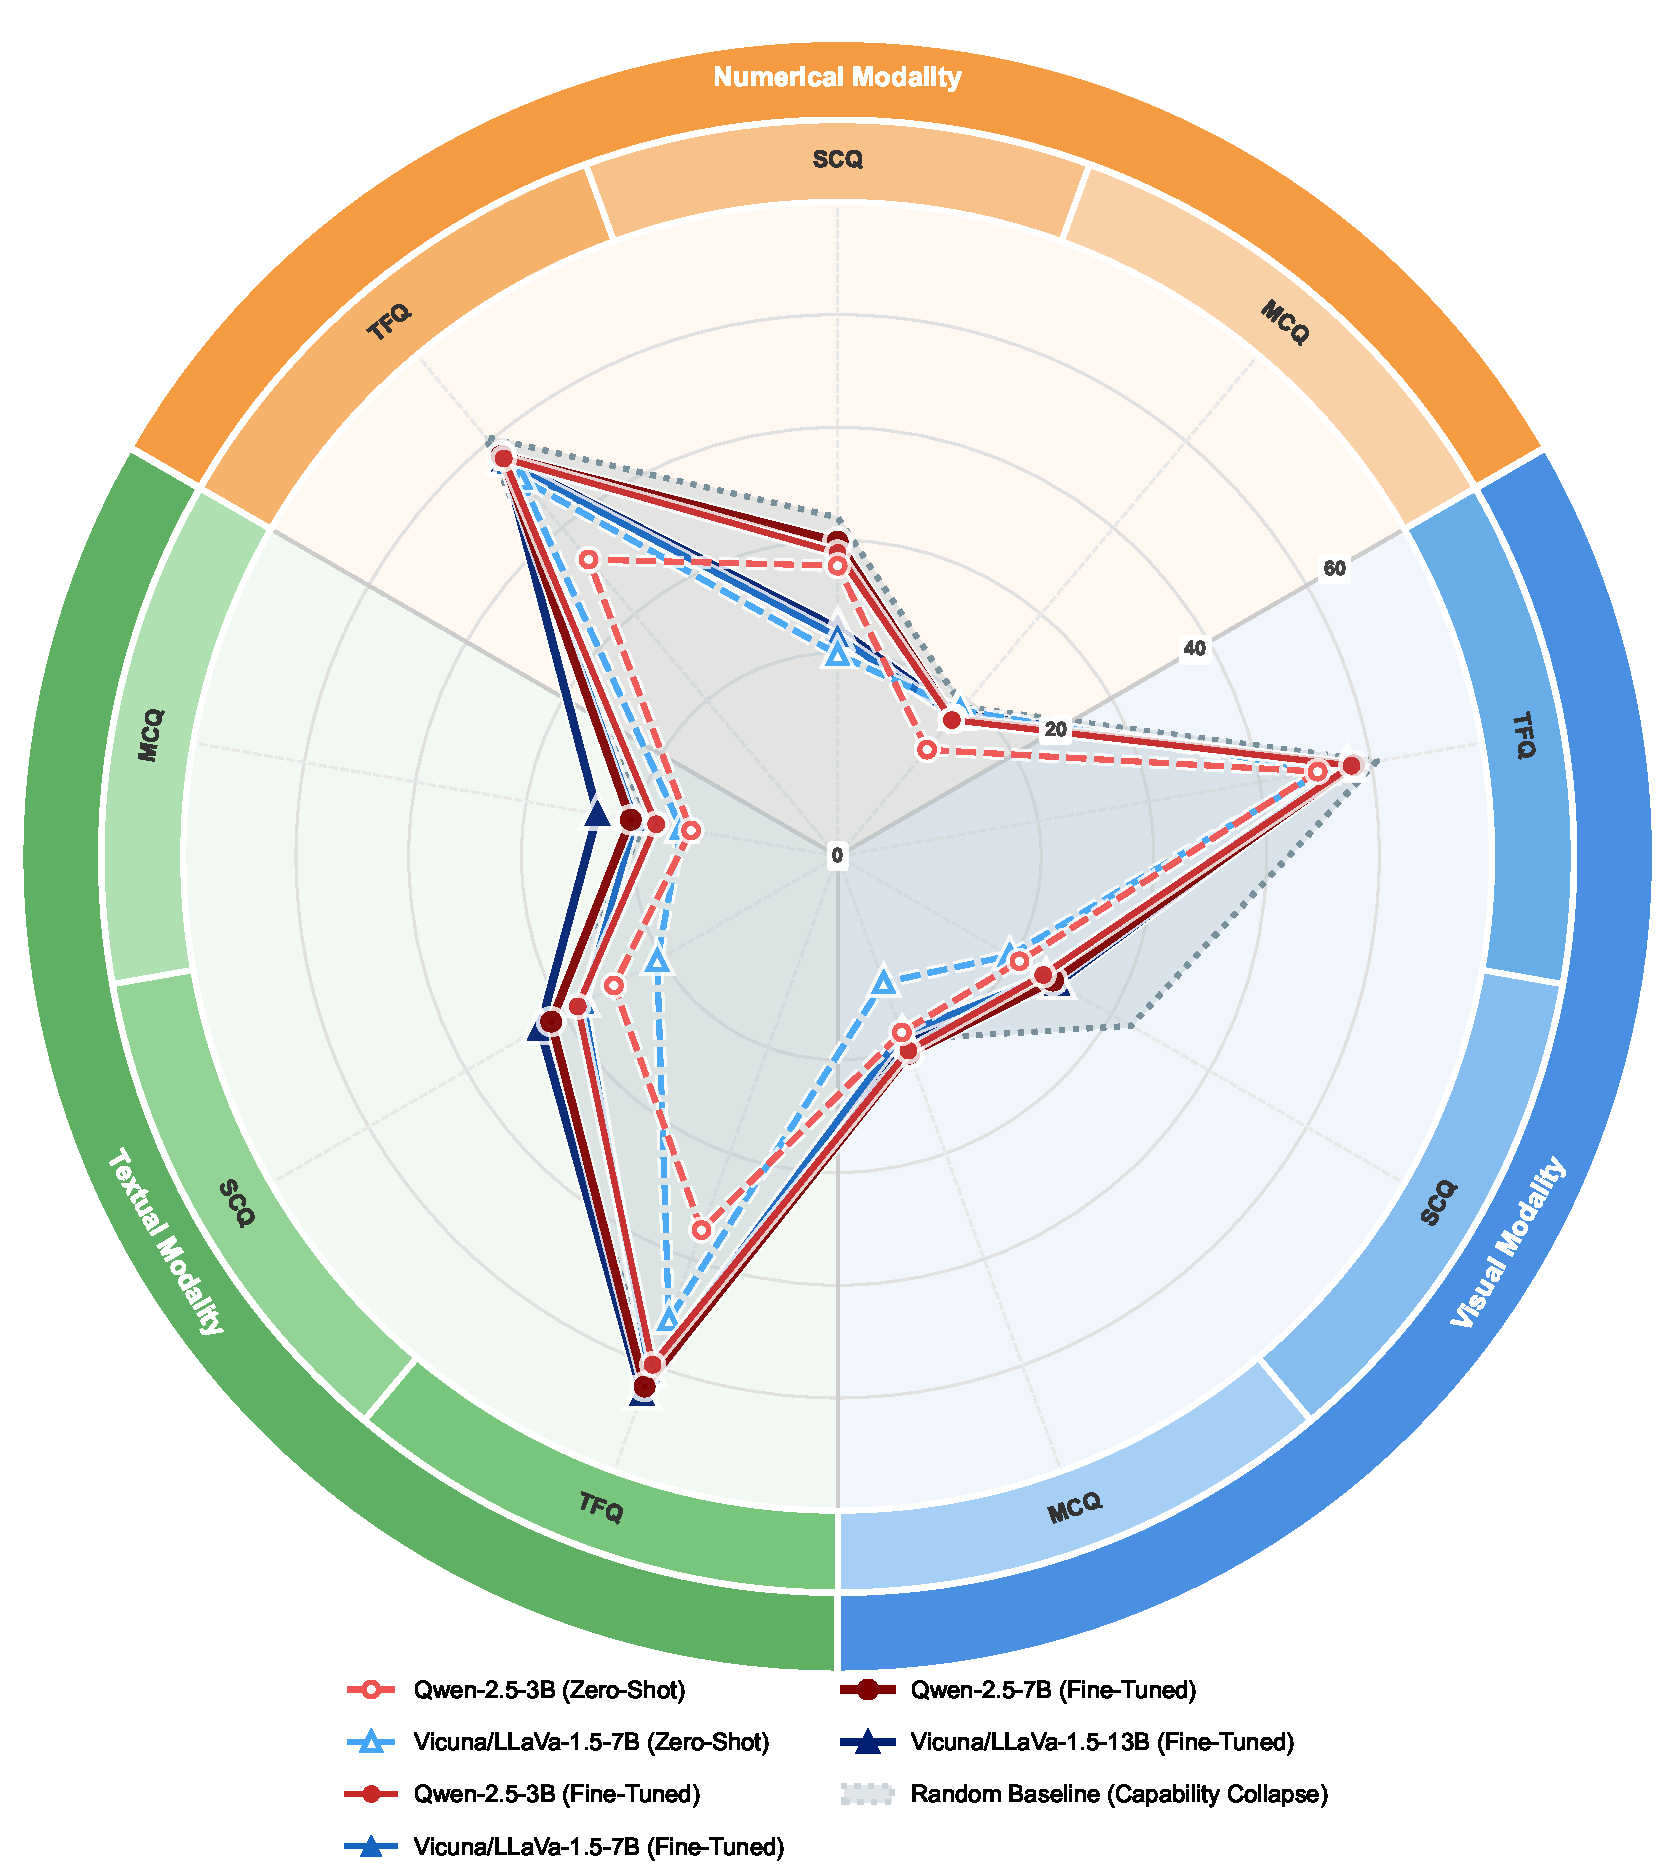
\includegraphics[width=\linewidth]{figure/figure3.pdf}
	\caption{Few-shot ablation in visual and numerical modalities (data from Experiment2). Colored reference lines indicate random-level thresholds for MCQ, SCQ, and TFQ. Performance fluctuations remain near random-level, showing no stable cognitive gain from additional demonstrations.}
	\label{fig:few_shot_ablation}
\end{figure}

\begin{figure*}[t!]
	\centering
	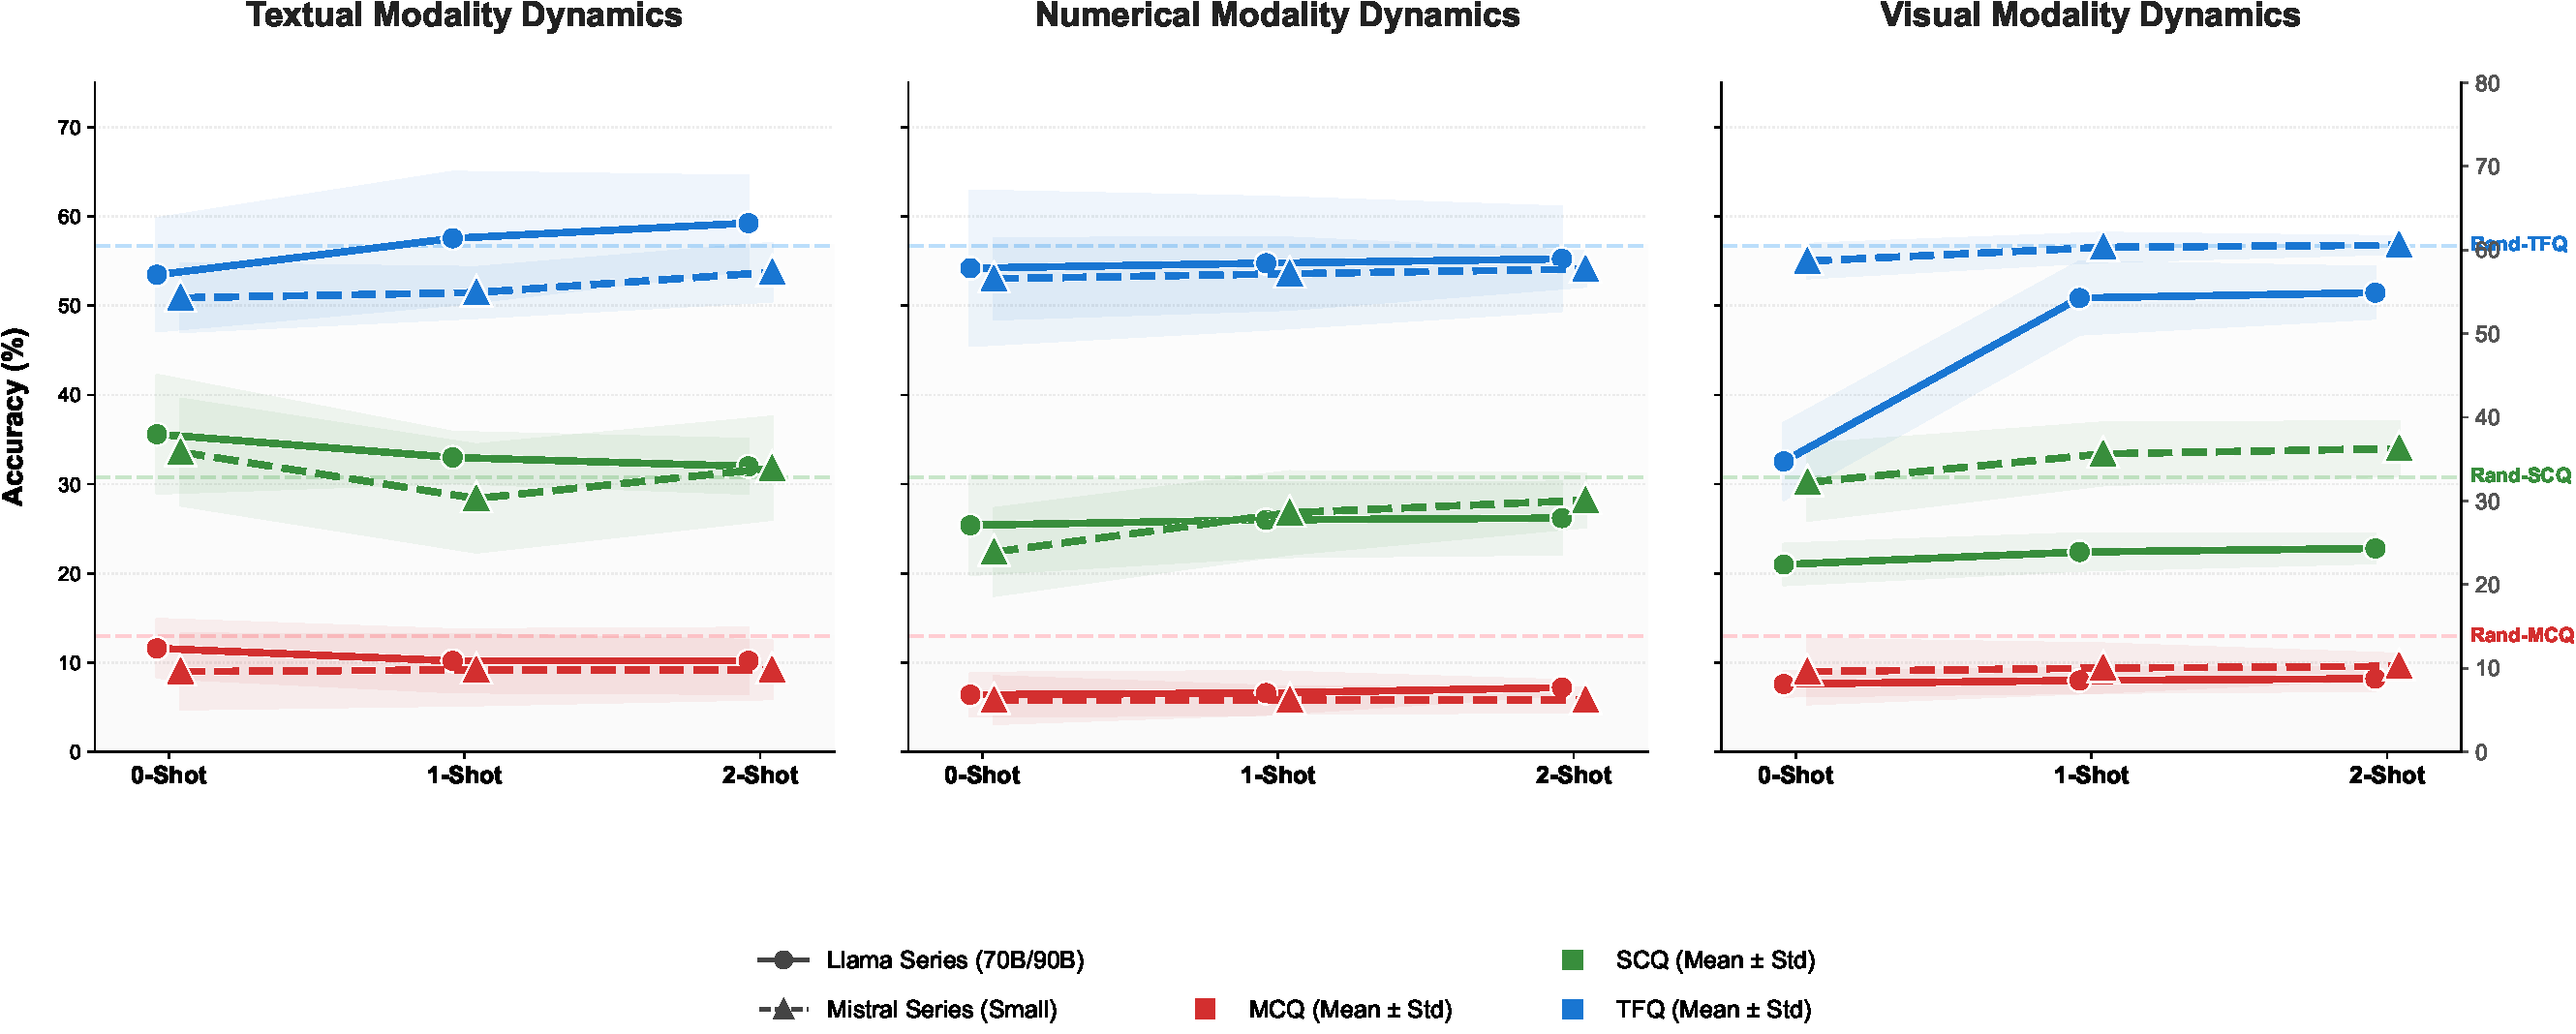
\includegraphics[width=\linewidth]{figure/figure4.pdf}
	\caption{Few-shot ablation in visual and numerical modalities (data from Experiment2). Colored reference lines indicate random-level thresholds for MCQ, SCQ, and TFQ. Performance fluctuations remain near random-level, showing no stable cognitive gain from additional demonstrations.}
	\label{fig:few_shot_ablation}
\end{figure*}



% \begin{figure}[t]
%     \centering
%     \fbox{
%         \parbox{0.95\linewidth}{
%         \textbf{Placeholder Figure: collapse severity across modalities.}\\
%         Suggested content: (x) models grouped by training setting; (y) collapse severity for Num and Vis, with an optional textual reference (prior HLC) for contrast; side-by-side or grouped bars.\\
%         Data: TBD.
%         }
%     }
%     \caption{Placeholder: collapse severity for non-semantic modalities (numerical and visual) in our main experiment, read together with textual HLC from prior work (tri-modal contrast).}
%     \label{fig:collapse_severity_placeholder}
% \end{figure}

% Finally, we relate collapse severity to parameter scale using the model families and sizes in Table~\ref{tab:main_results_hierarchical}. If collapse severity does not systematically decrease with scale (or behaves differently across Num vs.\ Vis), it rules out a purely ``more parameters fixes everything'' reading of Table~\ref{tab:main_results_hierarchical} and motivates the mechanistic follow-up in Section~\ref{sec:discussion}.

% \begin{figure}[t]
%     \centering
%     \fbox{
%         \parbox{0.95\linewidth}{
%         \textbf{Placeholder Figure: collapse severity vs parameter scale.}\\
%         Suggested content: scatter plot with x=scale (B) and y=collapse severity, colored by modality, with a simple regression trend line.\\
%         Data: TBD.
%         }
%     }
%     \caption{Placeholder: relationship between collapse severity and parameter scale (main experiment).}
%     \label{fig:collapse_scale_placeholder}
% \end{figure}